
\section{光滑与平展态射，及平坦性}

我们在前面已经定义过光滑\trMorphism{}与平展\trMorphism{}（\mbox{定义~13.6.2}），但直到现在，我们才真正有能力把它们的含义理解得透彻得多。我们将看到，\trUnramified{}态射这一概念（\S21.7）是它们的天然同伴。

我们的这三个代数几何定义，乍看之下并不明显是浑然一体的三胞胎；但我们将会讨论 [Gr-EGA] 中给出的定义（\S24.8.13），而在那套语境下，这三类态射看上去就非常相似了。（我们在 \S24.8.14 中还会简要提及其他的进路与定义。）

本章将要讨论的三类\trMorphism，是微分几何中下列几类流形之间的映射之类似物（参看 \S13.6.1）：
\begin{itemize}
\item \emph{\trSubmersion}是处处诱导\trTangentSpace{}之满射的映射。它们在\trFibration{}这一观念中很有用。（微分几何中或许更贴切、容许奇点的观念是：「在\trSource{}上局部地一个光滑纤维化」。）
\item \emph{在\trSource{}上局部的同构}（isomorphisms locally on the source，或称\emph{局部同构}，local isomorphisms）是诱导\trTangentSpace{}之同构的映射。
\item \emph{\trImmersion}是诱导\trTangentSpace{}之单射的映射。
\end{itemize}
（回想 \S9.2 中的警告：「浸入」一词在代数几何中常以别的含义使用。）

\begin{figure}[htbp]
\centering
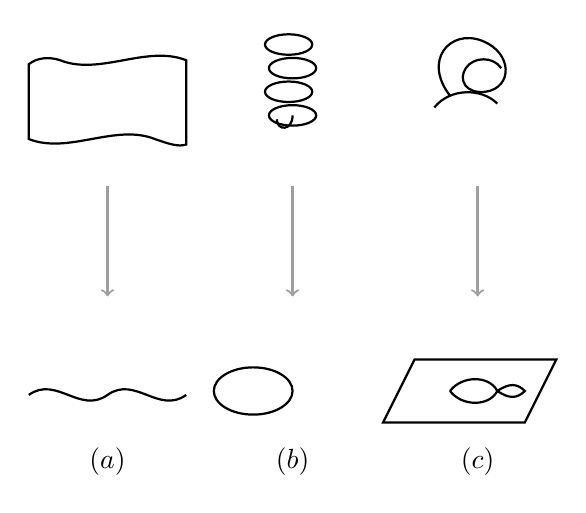
\begin{tikzpicture}[line width=0.8pt]
  \draw (0.0,4.35) .. controls (0.5,4.15) and (1.1,4.55) .. (1.6,4.35)
        .. controls (1.8,4.28) and (1.9,4.25) .. (2.0,4.28)
        -- (2.0,5.35) .. controls (1.5,5.55) and (0.9,5.15) .. (0.4,5.35)
        .. controls (0.25,5.4) and (0.1,5.38) .. (0.0,5.3) -- cycle;
  \draw[gray!75,->] (1.0,3.75) -- (1.0,2.35);
  \draw (0.0,1.1) .. controls (0.35,1.35) and (0.65,0.85) .. (1.0,1.1)
        .. controls (1.35,1.35) and (1.65,0.85) .. (2.0,1.1);
  \node at (1.0,0.25) {$(a)$};
  \draw (3.3,5.55) ellipse (0.30 and 0.13);
  \draw (3.35,5.25) ellipse (0.30 and 0.13);
  \draw (3.30,4.95) ellipse (0.30 and 0.13);
  \draw (3.35,4.65) ellipse (0.30 and 0.13);
  \draw (3.35,4.65) .. controls (3.35,4.45) and (3.15,4.45) .. (3.15,4.6);
  \draw[gray!75,->] (3.35,3.75) -- (3.35,2.35);
  \draw (2.85,1.15) ellipse (0.5 and 0.3);
  \node at (3.35,0.25) {$(b)$};
  \draw (5.35,4.9) .. controls (5.0,5.35) and (5.35,5.75) .. (5.75,5.6)
        .. controls (6.15,5.45) and (6.15,5.0) .. (5.8,4.95)
        .. controls (5.55,4.92) and (5.45,5.1) .. (5.55,5.25)
        .. controls (5.65,5.4) and (5.9,5.4) .. (6.0,5.25);
  \draw (5.15,4.75) .. controls (5.35,5.0) and (5.75,5.0) .. (5.95,4.8);
  \draw[gray!75,->] (5.7,3.75) -- (5.7,2.35);
  \draw (4.9,1.55) -- (6.7,1.55) -- (6.3,0.75) -- (4.5,0.75) -- cycle;
  \draw (5.35,1.15) .. controls (5.5,1.35) and (5.85,1.35) .. (5.95,1.15)
        .. controls (5.85,0.95) and (5.5,0.95) .. (5.35,1.15);
  \draw (5.95,1.15) .. controls (6.1,1.25) and (6.2,1.25) .. (6.3,1.15)
        .. controls (6.2,1.05) and (6.1,1.05) .. (5.95,1.15);
  \node at (5.7,0.25) {$(c)$};
\end{tikzpicture}
\caption{微分几何中诸观念的示意手绘：(a)「在\trSource{}上局部地一个光滑纤维化」的映射，(b) 局部同构，(c) 浸入。（代数几何中分别为：(a) 光滑\trMorphism，(b) 平展\trMorphism，(c) \trUnramified{}态射。）（依原书手绘图重绘。）}\label{fig:diffgeom-smooth-etale-unramified}
\end{figure}

为了更好地理解光滑\trMorphism{}与平展\trMorphism，我们暂时把先前给出的定义抛在脑后，转而考察一些例子：考察一些我们希望成为「局部同构」（或「在\trSource{}上局部地同构」，或「在\trSource{}上局部地一个光滑纤维化」）之类比的东西，看看它们能否帮助我们做出好的定义。

\textbf{24.8.1. 「局部同构」（平展\trMorphism）。}\quad 考虑复数域上抛物线 $x=y^2$ 到 $x$ 轴的投射。（这个例子以这样那样的形式反复出现过，\mbox{练习~13.6.F} 便是一例。）我们有理由希望它在原点之外是（\trSource{}上的）局部同构。我们或许还希望「局部同构」是个开条件型的观念：态射成为局部同构的那些点构成的\trLocus{}应当在\trSource{}上为开。就微分几何中的定义而言，事实的确如此。但这样一来，上述态射就应当在\trGenericPoint{}上是局部同构，而我们在\trGenericPoint{}处得到的是非平凡的\trResidueField{}\trFieldExtension{} $\mathbb{C}(y)/\mathbb{C}(y^2)$，并非\trIsomorphism。于是我们不得不把域的某些有限扩张（的诸 $\Spec$）也看作「\trSource{}上局部的同构」——在这个例子中，甚至是「覆盖空间」。（在\mbox{练习~24.8.D} 中我们将看到，我们想要的恰恰是有限可分扩张；这一点你其实早就能自己证明了。）

还要注意，在这个例子中，不存在非空的\trZariski{}开子集 $U\subset\Spec\mathbb{C}[x]\setminus\{0\}$ 与 $V\subset\Spec\mathbb{C}[x,y]/(x-y^2)\setminus\{(0,0)\}$，使得该映射把 $U$ 同构地送入 $V$（\mbox{练习~13.6.F}），所以这无论如何都不是你先前见过的某种意义下的局部同构。这便引出了\trEtale{}\trTopology{}这一观念——按通常的意义它甚至不是一张\trTopology，而是一个「\trGrothendieck{}\trTopology」（\S6.2.10）。平展\trTopology{}超出了本书的范围。

\textbf{24.8.2. \trSubmersion{}（光滑\trMorphism）。}\quad

\textbf{24.8.3.}\ \emph{纤维是光滑\trVariety。}\quad 作为淹没的代数几何版本的第一近似，我们希望诸\trFiber{}是（剩余域上的）光滑\trVariety。于是头一件需要做的事，就是把「\trVariety」这一观念推广到基上。给这条\trMorphism{}加上局部有限型假设，便可合理地做到这一点。由于某些颇为微妙的原因，我们将要求一个更强的条件：该\trMorphism{}是局部有限表现的。（如果你真想刨根问底，可以在我们的讨论中看到它在何处登场。当然，对诺特读者而言，两种说法没有差别。）

诸\trFiber{}不仅仅是\trVariety；它们还应当是\emph{光滑的}\trVariety（比如说，维数为 $n$）。由域上\trSmoothness{}的情形，或者由我们对光滑\trVariety{}应有的模样的直觉，可以期望\trFiber{}上的微分层是秩 $n$ 的\trLocallyFreeSheaf；更妙的是，可以期望相对微分层是秩 $n$ 的\trLocallyFreeSheaf。

\textbf{24.8.4.}\ \emph{\trFlatness。}\quad 至此，我们对「光滑\trMorphism」的第一近似是「局部有限表现，且纤维是光滑\trVariety」的某个版本。但这还不够。例如，从一个概形 $X$ 到一条\trCurve{} $Y$ 的一个糟糕的映射——它把一个互不相同的正则\trVariety{}送到 $Y$ 的每一点上（$X$ 是这些东西的无穷不交并）——在任何合理的意义下都不应被视为光滑纤维化。另外，我们或许也不想把 $\Spec k[\epsilon]/(\epsilon^2)\to\Spec k$ 视为淹没；比如说，它在\trTangentSpace{}上并非满射，而且更笼统地说，它的图像「看上去不像个纤维化」。

这两个问题都是 $\pi\colon X\to Y$ 未能成为一个良好的「连续」\trFamily{}的表现。凡是在寻找某种模糊的「良好性」观念时，我们都知道，「平坦性」将出现在定义之中。

作为对比，注意「\trUnramified」不含平坦性假设；我们也的确不曾指望它有——因为我们希望原点到 $\mathbb{A}^1$ 的包含（闭嵌入）是\trUnramified{}的。但这样一来，一些古怪的东西也可能是\trUnramified{}的。
\begin{figure}[htbp]
\centering
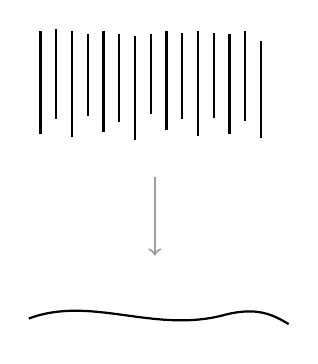
\begin{tikzpicture}[line width=0.8pt]
  \foreach \x/\h/\y in {0.55/1.30/0.00, 0.75/1.15/0.18, 0.95/1.35/-0.05,
    1.15/1.05/0.22, 1.35/1.28/0.02, 1.55/1.12/0.15, 1.75/1.32/-0.08,
    1.95/1.02/0.25, 2.15/1.25/0.05, 2.35/1.10/0.18, 2.55/1.33/-0.03,
    2.75/1.08/0.20, 2.95/1.27/0.00, 3.15/1.14/0.16, 3.35/1.24/-0.06} {
    \draw (\x,\y) -- (\x,\y+\h);
  }
  \draw[gray!75,->] (2.0,-0.55) -- (2.0,-1.55);
  \draw (0.4,-2.35) .. controls (1.2,-2.05) and (2.0,-2.55) .. (2.9,-2.3)
        .. controls (3.3,-2.2) and (3.5,-2.3) .. (3.7,-2.42);
\end{tikzpicture}
\caption{我们不想让这是一个「光滑\trMorphism」。（依原书手绘图重绘。）}\label{fig:not-want-smooth}
\end{figure}

例如，若 $X=\coprod_{z\in\mathbb{C}}\Spec\mathbb{C}$，则把对应于 $z$ 的那个点送到点 $z\in\mathbb{A}^1_{\mathbb{C}}$ 的\trMorphism{} $X\to\mathbb{A}^1_{\mathbb{C}}$ 是\trUnramified{}的。生活就是这样。

\textbf{24.8.5.}\ \emph{期望中的备选定义。}\quad 我们或许可以指望：态射 $\pi\colon X\to Y$ 是\textbf{相对维数 $n$ 光滑}的，当且仅当
（i）$\pi$ 局部有限表现，
（ii）$\pi$ 是相对维数 $n$ 的平坦，且
（iii）$\Omega_{X/Y}$ 是秩 $n$ 的局部自由层。
我们或许同样可以指望：态射 $\pi\colon X\to Y$ 是\textbf{平展}的，当且仅当
（i）$\pi$ 局部有限表现，
（ii）$\pi$ \trFlat，且
（iii）$\Omega_{X/Y}=0$。
我们很快就会证明（分别在\mbox{定理~24.8.8} 与\mbox{练习~24.8.C} 中）：这些期望中的定义与\mbox{定义~13.6.2} 等价。

\textbf{24.8.6. 光滑与平展\trMorphism{}的不同刻画。}\quad 本节的主要结果，是给出光滑\trMorphism{}的若干等价刻画，即\mbox{定理~24.8.8}。我们将先陈述该定理，随后给出它的若干推论，最后才给出证明。作为一条重要的前奏：

\textbf{24.8.7. \trhProposition。}\ ——\ \emph{光滑\trMorphism{}都是\trFlat{}的。}

\emph{证明。}\quad 我们先在诺特情形下证明。设 $\pi\colon X\to Y$ 是局部\trNoether{}概形之间的一个相对维数 $n$ 光滑的\trMorphism。我们希望证明它在一点 $p\in X$ 处平坦。由光滑\trMorphism{}的定义（\S13.6.2），不妨把 $X$ 与 $Y$ 分别换成 $p$ 与 $\pi(p)$ 的仿射邻域，使得 $\pi$ 成为态射
\[
\tag{24.8.7.1}\label{eq:smooth-affine-cover}
\Spec B[x_1,\dots,x_{n+r}]/(f_1,\dots,f_r)\longrightarrow\Spec B,
\]
而 $p$ 是\trJacobianMatrix{}满秩的一点。

\textbf{24.8.A.（练习）}\quad 用源上平坦性的\trSlicing{}判别法（\mbox{定理~24.6.9}）归纳地证明：
\[
\mathbb{A}^{n+r}_{B}\supset V(f_1)\supset V(f_1,f_2)\supset\cdots\supset V(f_1,\dots,f_r)=X
\]

这些概形都在 $p$ 处于 $B$ 上光滑且平坦，从而在诺特情形下证明了\mbox{命题~24.8.7}。（你将需要「光滑 $k$-概形既约」这一事实，\mbox{命题~13.2.13}。）

（诺特读者可以得意洋洋地直接跳到证明的末尾。）我们用一个狡猾的招数来证明一般情形。我们仍把 $\pi$ 局部地写成 \eqref{eq:smooth-affine-cover}。通过重新安排诸 $x$-变量的次序，不妨假设 $f_1,\dots,f_r$ 关于前 $r$ 个变量 $x_1,\dots,x_r$ 的\trJacobianMatrix{}是可逆的。设
\[
f_i(x_1,\dots,x_{n+r})=\sum_{a^i_1,\dots,a^i_{n+r}}b^i_{a^i_1,\dots,a^i_{n+r}}\,x_1^{a^i_1}\cdots x_{n+r}^{a^i_{n+r}},
\]
其中 $b^i_{j,\dots,k}\in B$。（这些都是有限和！）考虑多项式代数 $P=\mathbb{Z}[c^i_{j,\dots,k}]$，其中诸 $c$-变量的指标恰好取诸 $b$-变量的指标中出现过的那些。定义 $g_i\in P[x_1,\dots,x_{n+r}]$ 如下：
\[
g_i(x_1,\dots,x_{n+r})=\sum_{a^i_1,\dots,a^i_{n+r}}c^i_{a^i_1,\dots,a^i_{n+r}}\,x_1^{a^i_1}\cdots x_{n+r}^{a^i_{n+r}}.
\]
设 $J\in P[x_1,\dots,x_{n+r}]$ 是 $g_1,\dots,g_r$ 关于 $x_1,\dots,x_r$ 的\trJacobianMatrix{}的行列式。最后，令 $R:=P_J$。我们有一张\trCartesianDiagram
\[
\begin{tikzcd}[row sep=3.2em, column sep=6.5em]
\Spec B[x_1,\dots,x_{n+r}]/(f_1,\dots,f_r) \ar[r] \ar[d, "\pi"'] & \Spec R[x_1,\dots,x_{n+r}]/(g_1,\dots,g_r) \ar[d, "\alpha"] \\
\Spec B \ar[r] & \Spec R
\end{tikzcd}
\]
它把 $c^i_{j,\dots,k}$ 送到 $b^i_{j,\dots,k}$，并把 $g_i$ 送到 $f_i$。由于 $J$ 在 $R$ 中可逆，$\alpha$ 是相对维数 $n$ 光滑的（基本上就是定义）。由这一结果已证的诺特情形，$\alpha$ 是\trFlat{}的。而平坦性在\trBaseChange{}下保持，故 $\pi$ \trFlat，正如所愿。\hfill$\square$

现在我们来到本节的中心结果。

\textbf{24.8.8. \trhTheorem。}\ ——\ \emph{设 $\pi\colon X\to Y$ 是概形之间的一个\trMorphism。则下列诸条等价。}
（i）\emph{\trMorphism{} $\pi$ 是相对维数 $n$ 光滑的（\mbox{定义~13.6.2}）。}
（ii）\emph{\trMorphism{} $\pi$ 局部有限表现且是相对维数 $n$ 的平坦；并且 $\Omega_\pi$ 是秩 $n$ 的局部自由层（\mbox{期望中的备选定义~24.8.5}）。}
（iii）\emph{\trMorphism{} $\pi$ 局部有限表现且\trFlat，并且诸\trFiber{}是纯维数 $n$ 的光滑 $k$-概形。}
（iv）\emph{\trMorphism{} $\pi$ 局部有限表现且\trFlat，并且诸几何纤维是纯维数 $n$ 的光滑 $k$-概形。}

我们先把这条定理中那些基本上已经证明过的部分解决掉。

\textbf{24.8.B.（练习）}\quad 证明 (i) 蕴涵 (ii) 蕴涵 (iii)，并证明 (iii) 与 (iv) 等价。提示（依次为）：光滑蕴涵平坦，用\mbox{命题~24.8.7}；以微分给出的光滑 $k$-\trVariety{}的定义，见\mbox{重新定义~21.2.28}；\trSmoothness{}与域扩张无关，用\mbox{练习~13.2.H}。

在 \S24.8.11 中完成\mbox{定理~24.8.8} 的证明之前，我们先给出若干道练习与几条假定它成立的结果，以期为这一结果提供动机。

\textbf{24.8.C.（练习）}\quad 证明：态射 $\pi$ 是平展的（\mbox{定义~13.6.2}），当且仅当 $\pi$ 局部有限表现、\trFlat，并且 $\Omega_\pi=0$（\mbox{期望中的备选定义~24.8.5}）。

\textbf{24.8.D.（容易练习）}\quad 设 $\pi\colon X\to Y$ 是一个\trMorphism。证明下列诸条等价。
（a）$\pi$ 平展。
（b）$\pi$ 光滑且\trUnramified。
（c）$\pi$ 局部有限表现、平坦且\trUnramified。
（d）$\pi$ 局部有限表现、平坦，并且对每个 $q\in Y$，$\pi^{-1}(q)$ 都是形如 $\Spec K$ 的概形的不交并，其中 $K$ 是 $\kappa(q)$ 的一个有限可分扩张。
（e）$\pi$ 局部有限表现、平坦，并且对 $Y$ 的每个\emph{\trGeometricPoint}{} $\overline{q}$，$\pi^{-1}(\overline{q})$ 都是若干份 $\overline{q}$ 拷贝的不交并。

\textbf{24.8.E.（重要练习）}\quad 设 $\pi\colon X\to Y$ 平展。证明：局部环维数为 $n$ 的正则点 $q\in Y$ 在 $X$ 中的任何原像 $p\in X$，也是一个局部环维数为 $n$ 的正则点。提示：对 $\dim\OO_{Y,q}$ 作归纳来证明本结果。用 $\mathfrak{m}_{Y,q}\setminus\mathfrak{m}_{Y,q}^2$ 中的元素「切片」。用正则性的\trSlicing{}判别法（\mbox{练习~13.2.C}）。

\textbf{24.8.9.}\ \emph{光滑性--正则性比较\mbox{定理~13.2.7(b)} 的证明（每个光滑 $k$-概形都正则）。}\quad 由\mbox{观察~13.6.4}，任何维数 $n$ 的光滑 $k$-概形 $X$ 在局部上都可以写成 $\mathbb{A}^n_k$ 的一个平展覆盖，而后者是正则的（\mbox{练习~13.3.P}）。再由\mbox{练习~24.8.E}，$X$ 是正则的。\hfill$\square$

\textbf{24.8.F.（练习）}\quad 设 $\pi\colon X\to Y$ 是纯维 $k$-\trVariety{}之间的一个\trMorphism，而 $Y$（在 $k$ 上）光滑。用余切正合列（\mbox{定理~21.2.24}）证明下列两条。
（a）设 $\dim X=\dim Y=n$，且 $\pi$ \trUnramified。证明 $X$ 光滑。
（b）设 $\dim X=m>\dim Y=n$，且 $\pi$ 在闭点之上的（概形论）\trFiber{}都是维数 $m-n$ 的光滑概形。证明 $X$ 光滑。

\textbf{24.8.G.（练习）}\quad 设 $\pi\colon X\to Y$ 是光滑纯维 $k$-\trVariety{}之间的一个（$k$ 上的）\trMorphism，其中 $\dim X=m$、$\dim Y=n$。（两个小题显然本质上是同一几何情势。）
（a）证明：若 $\pi$ 的诸\trFiber{}都是维数 $m-n$ 的光滑概形，则 $\pi$ 是相对维数 $m-n$ 光滑的。
（b）证明：若 $\pi^*\Omega_Y\to\Omega_X$ 是「向量丛的单射」（见\mbox{定义~14.2.4}），或者等价地说，「$T_\pi$ 是满射」，则 $\pi$ 是相对维数 $m-n$ 光滑的。
可能的进路：对每一点 $q\in Y$，$\OO_{Y,q}$ 都是一个正则局部环。对 $\dim\OO_{Y,q}$ 作归纳，并用 $\mathfrak{m}_{Y,q}\setminus\mathfrak{m}_{Y,q}^2$ 中的元素「切片」。

\textbf{24.8.10.}\ \emph{\trhRemark。}\quad 设 $\pi\colon X\to Y$ 局部有限表现，$\rho\colon Y\to Z$ 平展，而 $\tau=\rho\circ\pi$。则 $\pi$ 是维数 $n$ 光滑的（例如取 $n=0$ 即平展），当且仅当 $\tau$ 也是。一个方向是\mbox{练习~13.6.D}，另一个方向是\mbox{练习~21.7.G}(b)。类似地，$\pi$ \trUnramified{}当且仅当 $\tau$ \trUnramified{}（\mbox{练习~21.7.C} 与\mbox{练习~21.7.G}(a)）。

\textbf{24.8.11.}\ \extrahard\ \emph{\mbox{定理~24.8.8} 的证明。}\quad 由\mbox{练习~24.8.B}，只剩下证明 (iii) 蕴涵 (i)。（这一论证使人想起\mbox{定理~13.6.6} 的证明。）

取定一个闭点 $p\in X$，并令 $q=\pi(p)\in Y$。我们将证明：存在 $p$ 的一个开邻域 $U_i$ 与 $q$ 的一个开邻域 $V_i$，具有\mbox{定义~13.6.2} 中所述的形状。只须处理 $p$ 是 $\pi^{-1}(q)$ 中闭点的情形，因为闭点在有限型概形中稠密（\mbox{练习~5.3.F}）。（然而，我们不能假设 $q$ 是 $Y$ 的闭点。）

由于 $\pi$ 有限表现，存在 $p$ 的仿射开邻域 $U\subset X$ 与 $q$ 的仿射开邻域 $V\subset Y$，满足 $\pi(U)\subset V$，使得\trMorphism{} $\pi|_U\colon U\to V$ 可以写成
\[
U=\Spec B[x_1,\dots,x_N]/I\ \xrightarrow{\ \pi|_U\ }\ \Spec B=V,
\]
其中 $I$ 有限生成。取 $\overline{I}$ 的一组生成元 $\overline{f}_1,\dots,\overline{f}_s$。考虑\trCartesianDiagram
\[
\begin{tikzcd}[row sep=2.6em, column sep=4.6em]
\overline{U} \ar[r, hook] \ar[d, equals] & U \ar[d, equals] \\
\Spec\kappa(q)[x_1,\dots,x_N]/\overline{I} \ar[r, hook] \ar[d] & \Spec B[x_1,\dots,x_N]/I \ar[d, "\pi|_U"'] \\
\Spec\kappa(q) \ar[r, hook] \ar[d, equals] & \Spec B \ar[d, equals] \\
q \ar[r, hook] & V,
\end{tikzcd}
\]
其中 $\overline{U}$ 是 $U$ 在 $q$ 之上的\trFiber，而 $\overline{I}$ 是在 $\mathbb{A}^N_{\kappa(q)}$ 中切出 $\overline{U}$ 的那个理想。

回想 \S24.2.2：对平坦于基的闭子概形而言，把定义理想拉回（作为拟凝聚层）所得者，与拉回后的闭子概形的理想相同。于是，由于 $B[x_1,\dots,x_N]/I$ 在 $B$ 上平坦，我们有 $\overline{I}=I\otimes_B\kappa(q)$。从而 $\overline{f}_1:=f_1\otimes 1,\ \dots,\ \overline{f}_s:=f_s\otimes 1$ 生成 $I\otimes_B\kappa(q)=\overline{I}$。

由假设 (iii)，\trFiber{} $\overline{U}\subset\mathbb{A}^N_{\kappa(q)}$ 在 $\kappa(q)$ 上光滑，故 $\OO_{\overline{U},p}$ 是一个维数为 $n$ 的\trIntegralDomain（\mbox{练习~13.2.O}）。仍由假设 (iii)，$\overline{f}_1,\dots,\overline{f}_s$（关于 $x_1,\dots,x_N$）的\trJacobianMatrix{}在 $p$ 处的余秩为 $n$，也就是说，该\trJacobianMatrix{}的秩为 $r:=N-n$。于是我们可以给诸 $\overline{f}_i$ 重新命名，使得其中\emph{前} $r$ 个 $\overline{f}_1,\dots,\overline{f}_r$ 的\trJacobianMatrix{}在 $p$ 处余秩为 $n$。于是 $\overline{U}':=\Spec\kappa(q)[x_1,\dots,x_N]/(\overline{f}_1,\dots,\overline{f}_r)$ 在 $\kappa(q)$ 上相对维数 $n$ 光滑（在 $p$ 的某个邻域内），故 $\OO_{\overline{U}',p}$ 是维数为 $n$ 的\trIntegralDomain（再次用\mbox{练习~13.2.O}）。

于是
\[
\OO_{\overline{U}',p}\twoheadrightarrow\OO_{\overline{U}',p}/(\overline{f}_{r+1},\dots,\overline{f}_s)=\OO_{\overline{U},p}
\]
\begin{figure}[htbp]
\centering
\begin{tikzpicture}[line width=0.8pt,font=\small]
  \draw (1.5,3.5) .. controls (3.0,3.3) and (4.5,3.7) .. (6.35,3.45)
        -- (6.45,4.5) .. controls (4.6,4.75) and (3.0,4.3) .. (1.6,4.55) -- cycle;
  \node[align=center,font=\footnotesize] at (3.98,4.12)
    {$U'\overset{\text{开}}{\subset}\Spec R$\\
     $=\Spec B[x_1,\dots,x_n]/(f_1,\dots,f_r)$};
  \draw (1.25,1.95) .. controls (3.0,1.7) and (4.8,2.15) .. (6.6,1.85)
        -- (6.5,3.35) .. controls (4.7,3.65) and (3.0,3.15) .. (1.35,3.45) -- cycle;
  \node at (4.05,3.12) {$U=\Spec R/J$};
  \node[align=center,font=\footnotesize] at (4.05,2.6)
    {$=\Spec B[x_1,\dots,x_n]$\\
     $/(f_1,\dots,f_r,\dots,f_s)$};
  \fill (1.6,1.98) circle (2.0pt);
  \node[anchor=west] at (1.7,1.98) {$p=\Spec\kappa(p)$};
  \draw[line width=0.7pt] (0.7,4.55) .. controls (0.9,4.55) and (0.8,4.15)
        .. (0.96,3.77) -- (0.83,3.65) -- (0.96,3.53)
        .. controls (0.8,3.1) and (0.9,2.05) .. (0.7,1.9);
  \node[anchor=east] at (0.64,3.2) {$\overline{U}'$};
  \draw[line width=0.7pt] (0.88,3.33) .. controls (1.06,3.33) and (0.97,3.0)
        .. (1.12,2.67) -- (1.0,2.55) -- (1.12,2.43)
        .. controls (0.97,2.1) and (1.06,1.77) .. (0.88,1.55);
  \node[anchor=east] at (0.82,2.45) {$\overline{U}$};
  \draw[gray!75,->] (4.0,1.5) -- (4.0,0.75);
  \fill (1.0,0.3) circle (2.0pt);
  \draw (1.0,0.3) -- (6.55,0.3);
  \node[anchor=north] at (1.4,0.1) {$q=\Spec\kappa(q)$};
  \node[anchor=north] at (5.1,0.22) {$V=\Spec B$};
\end{tikzpicture}
\caption{\mbox{定理~24.8.8} 部分证明背后的几何。（依原书手绘图重绘。）}\label{fig:geometry-smooth-proof}
\end{figure}

这是两个维数同为 $n$ 的\trIntegralDomain{}之间的一个满射，从而由\mbox{容易练习~13.2.M}，它是一个\trIsomorphism。于是 $\overline{U}=\overline{U}'$ 在 $\overline{U}$ 中 $p$ 附近成立（更精确地说，存在 $\overline{U}$ 中 $p$ 的一个邻域，它同时也是 $\overline{U}'$ 中 $p$ 的一个邻域）。

设 $U'\subset\Spec B[x_1,\dots,x_N]/(f_1,\dots,f_r)$ 是使 $f_1,\dots,f_r$（关于 $x_1,\dots,x_N$）的\trJacobianMatrix{}余秩为 $n$（即满秩 $r$）的那个开子集。那么由定义，$U'\to\Spec B$ 是相对维数 $n$ 光滑的。我们将证明：存在 $U$ 中 $p$ 的一个邻域，它同时也是 $U'$ 中 $p$ 的一个邻域，从而完成证明。

为方便起见，令 $R:=B[x_1,\dots,x_N]/(f_1,\dots,f_r)$\footnote{原书此处作「$B[x_1,\dots,x_n]$」，惟本证明通篇记变元数为 $N$（如 $\mathbb{A}^N_{\kappa(q)}$、余秩计算），当为「$x_N$」之误，径改。——译者注}，并令 $J:=(f_{r+1},\dots,f_s)\subset R$（见图~\ref{fig:geometry-smooth-proof}）。由于 $J$ 是一个有限生成的理想，它支撑在 $\Spec R$ 的一个闭子集上（\mbox{练习~6.6.B}(b)）。我们希望证明：$p$ 不在 $\Spec R$ 中 $J$ 的支撑之内。由\trNakayama{}引理，只须证明 $J\otimes_R\kappa(p)=0$。

由于 $U=\Spec R/J\subset X$ 在 $B$ 上光滑，$R/J$ 在 $B$ 上平坦（\mbox{命题~24.8.7}）。现在，$J\otimes_B\kappa(q)$ 是在 $\overline{U}'$ 中切出 $\overline{U}$ 的那个理想（再次用 \S24.2.2，这里用到 $U=\Spec R/J$ 的平坦性）\footnote{译注：原书此处作「the ideal cutting out $\overline{U}'$ in $\overline{U}$」；按 \S24.8.11 的记号，$\overline{U}$ 是 $\overline{U}'$ 中由 $\overline{f}_{r+1},\dots,\overline{f}_s$ 切出的闭子概形，故当为「cutting out $\overline{U}$ in $\overline{U}'$」之误，径改。——译者注}，而 $\overline{U}=\overline{U}'$ 在 $\overline{U}$ 中 $p$ 附近成立。于是 $J\otimes_B\kappa(q)$ 在 $p$ 附近为零（也就是说，在 $p$ 的某个开邻域内 $J\otimes_B\kappa(q)=0$），从而 $(J\otimes_B\kappa(q))\otimes_R\kappa(p)=0$。那么
\[
J\otimes_R\kappa(p)=J\otimes_R(\kappa(p)\otimes_B\kappa(q))=(J\otimes_B\kappa(q))\otimes_R\kappa(p)=0,
\]
正如所愿。\hfill$\square$

\textbf{24.8.12.}\ \extrahard\ \textbf{形式\trUnramified、形式\trSmooth{}与形式\trEtale。}\quad [Gr-EGA] 为\trUnramified、\trSmooth{}与\trEtale{}态射的定义选取了另一个出发点。那里的定义清楚地表明：这三个定义构成一个家族。

这些定义的代价在于：它们在几何上的直接动机或许要弱一些，而且证明某些基本性质也更加困难。其好处则是：能够证明的东西更多了（例如，余切正合列与余正规正合列的左正合性，以及借助局部环的完备化给出的良好解读）。但我们在这里只是引入这些想法，而不去探讨它们。参看
[BLR, \S2.2]——那里有一份出色的讨论。（下述内容你大可以置之不理，除非日后你发现自己当真在乎。）

\textbf{24.8.13.}\ \emph{\trhDefinition。}\quad 我们说 $\pi\colon X\to Y$ 是\textbf{形式\trSmooth}（formally smooth）的（相应地，\textbf{形式\trEtale}（formally étale）的、\textbf{形式\trUnramified}（formally unramified）的），如果对一切仿射概形 $Z$、每个由幂零理想定义的闭子概形 $Z_0\subset Z$ 以及每个态射 $Z\to Y$，典范映射 $\Hom_Y(Z,X)\to\Hom_Y(Z_0,X)$ 都是满射（相应地，双射、单射）。下面的交换图概括了这一点，它使人想起分离性与固有性的\trValuativeCriteria：
\[
\begin{tikzcd}[row sep=3.2em, column sep=4.2em]
Z_0 \ar[r] \ar[d, "\text{幂零理想}"'] & X \ar[d, "\pi"] \\
Z \ar[r] \ar[ur, dashed, "?"'] & Y
\end{tikzcd}
\]
（你可以检验：若把「幂零」换成「平方为零」，得到的定义与此相同。这种表述有时用起来更容易。）于是 [Gr-EGA] 把「光滑」定义为形式光滑且局部有限表现的态射，\trUnramified{}与平展的情形类似。

可以证明，[Gr-EGA] 给出的形式\trUnramified{}与形式\trSmooth{}的定义与我们给出的定义相一致。关于「形式\trUnramified」（我们在 \S21.7 中给出的定义并不显然与这里所引 [Gr-EGA] 的定义相同），见 [Gr-EGA, IV$_4$.17.2.1] 或 [Stacks, tag~00UO]；关于「光滑」，见 [Gr-EGA, IV$_4$.17.5.1] 或 [Stacks, tag~00TN]。（我们把平展刻画为相对维数 $0$ 光滑，这与 [Gr-EGA] 相一致。而我们把\trUnramified{}定义为形式\trUnramified{}加上局部有限\emph{型}，则与 [Gr-EGA] 不一致，如 \S21.7 中所述。）

\textbf{24.8.14. 其他的出发点。}\quad 定义光滑、平展与\trUnramified{}态射的方式相当之多，而且要把它们彼此联系起来也绝非平凡。我们刚刚描述了 [Gr-EGA] 的进路。另一种常见的进路，是把光滑态射刻画为局部有限表现、平坦、且几何纤维正则的态射（见\mbox{定理~24.8.8}）。还有一种定义则是通过余切复形的朴素版本；这正是 [Stacks, tag~00T2] 所采取的进路，而且并不像听起来那么吓人。最后，\mbox{练习~24.8.D} 中那些不同的刻画，也给出了平展性的一些备选的初始定义。
